\section{Compiler Options}
The compiler options tested where:
\begin{itemize}
\item \textbf{none} No optimization
\item \textbf{-xO1 to -xO5} Different levels of optimization. The higher the number the more aggressively the compiler tries to optimiz the code for performance.
\item \textbf{-xrestrict} Treats pointer-valued function parameters as restricted pointers. A restricted pointers are assumed not to be aliased. This flag improves vectorization.
\item \textbf{-fast} Macro that applies various options including -xO5. 
\end{itemize}
The different options was tested for different memory footprints on both an the AMD and Intel CPU. The results are given on figure \ref{fig:compilerOptionsAmd} and \ref{fig:compilerOptionsIntel}.
\begin{figure}[here]
\centering
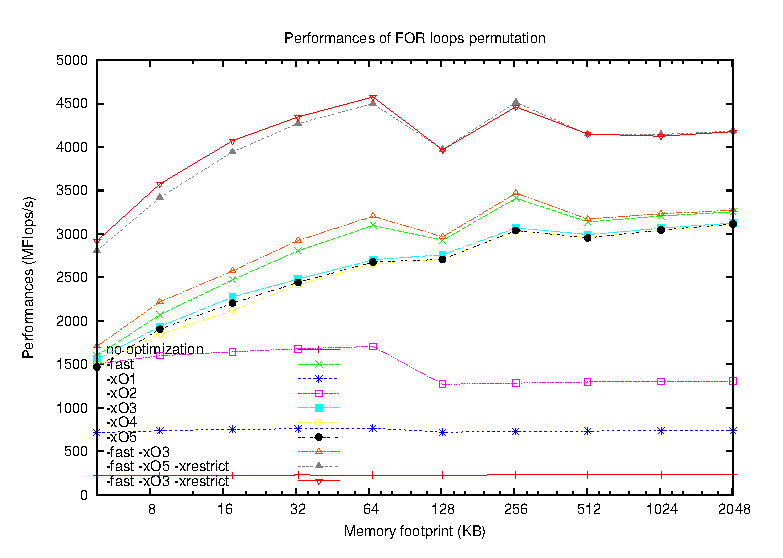
\includegraphics[width=0.8\textwidth]{results/flag-test-plot-intel.eps}
\caption{Timings of different compiler options on the intel CPU}
\label{fig:compilerOptionsIntel}
\end{figure}
\begin{figure}[here]
\centering
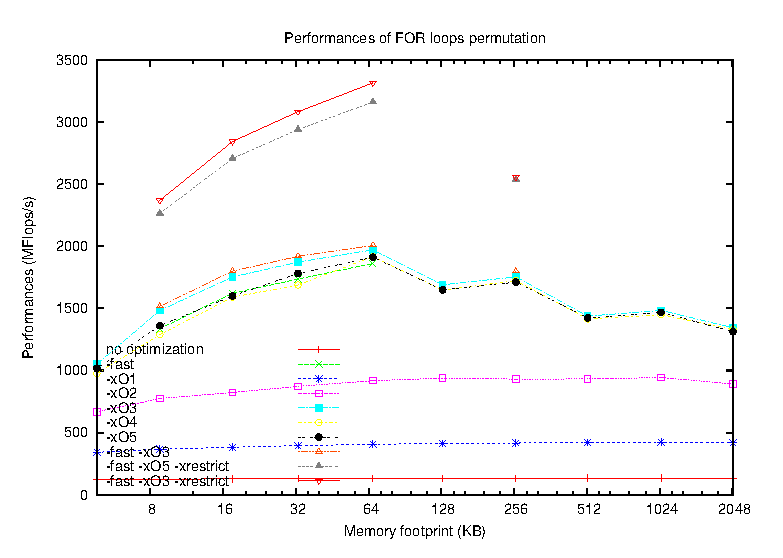
\includegraphics[width=0.8\textwidth]{results/flag-test-plot-amd.eps}
\caption{Timings of different compiler options on the AMD CPU}
\label{fig:compilerOptionsAmd}
\end{figure}
\\\\
The fastest set of options on both the AMD and Intel is -fast -xO3 -xrestrict. The missing data points on figure \ref{fig:compilerOptionsAmd} is because test failed because of a compiler error whenever -fast. 
\\\\
As it can be seen from figure \ref{fig:3way} and figure \ref{fig:compilerOptionsIntel} that even though we use the fastest options we cannot compile a version of our implementation that is faster than the library function. 
\\\\
It is also interesting to note that options -x04 and -x05 performs worse than -xO3 on both the Intel and AMD. 